\documentclass{article}

\usepackage{amsmath}
\usepackage{graphicx}

\graphicspath{ {./assets/} }

\setlength\paperwidth{20.999cm}\setlength\paperheight{29.699cm}\setlength\voffset{-1in}\setlength\hoffset{-1in}\setlength\topmargin{1.499cm}\setlength\headheight{12pt}\setlength\headsep{0cm}\setlength\footskip{1.131cm}\setlength\textheight{25cm}\setlength\oddsidemargin{2.499cm}\setlength\textwidth{15.999cm}

\begin{document}
\begin{center}
\hrule

\vspace{.4cm}
{\bf {\Huge Assignment 4}} \\
\vspace{.2cm}
{\bf Computer Graphics}
\vspace{.2cm}
\end{center}
{\bf Edoardo Riggio } (edoardo.riggio@usi.ch) \hspace{\fill}  \today \\
\hrule
\vspace{.2cm}

\section{Exercise 1}
\subsection{Task 1}
The two matrices $R_90$ and $T$ in homogeneous coordinates are as follows:
\[ R_{90} = \begin{bmatrix} 1 & 0 & 1 \\ 0 & 1 & -2 \\ 0 & 0 & 1 \end{bmatrix} \]
\[ T = \begin{bmatrix} \cos{90} & -\sin{90} & 0 \\ \sin{90} & \cos{90} & 0 \\ 0 & 0 & 1 \end{bmatrix} = \begin{bmatrix} 0 & -1 & 0 \\ 1 & 0 & 0 \\ 0 & 0 & 1 \end{bmatrix} \]

\subsection{Task 2}
The following are the computations for the rotated and translated points and vector:
\begin{align*}
	p'_1 & =  \begin{bmatrix}1&0&1\\ 0&1&-2\\0&0&1\end{bmatrix} \left( \begin{bmatrix}0&-1&0\\ 1&0&0\\ 0&0&1\end{bmatrix}\begin{bmatrix}1\\ 1\\ 1\end{bmatrix} \right)  =  \begin{bmatrix}1&0&1\\ 0&1&-2\\0&0&1\end{bmatrix}\begin{bmatrix}0\cdot 1+\left(-1\right)\cdot 1+0\cdot 1\\ 1\cdot 1+0\cdot 1+0\cdot 1\\ 0\cdot 1+0\cdot 1+1\cdot 1\end{bmatrix} \\
	& = \begin{bmatrix}1&0&1\\ 0&1&-2\\0&0&1\end{bmatrix}\begin{bmatrix}-1\\ 1\\ 1\end{bmatrix} = \begin{bmatrix}1\cdot \left(-1\right)+0\cdot 1+1\cdot 1\\ 0\cdot \left(-1\right)+1\cdot 1+\left(-2\right)\cdot 1\\ 0\cdot \left(-1\right)+0\cdot 1+1\cdot 1\end{bmatrix} = \begin{bmatrix}0\\ -1\\ 1\end{bmatrix} \mapsto \begin{bmatrix}0\\ -1\end{bmatrix}
\end{align*}

\begin{align*}
	p'_2 & =  \begin{bmatrix}1&0&1\\ 0&1&-2\\0&0&1\end{bmatrix} \left( \begin{bmatrix}0&-1&0\\ 1&0&0\\ 0&0&1\end{bmatrix}\begin{bmatrix}3\\ 2\\ 1\end{bmatrix} \right)  =  \begin{bmatrix}1&0&1\\ 0&1&-2\\0&0&1\end{bmatrix}\begin{bmatrix}0\cdot 3+\left(-1\right)\cdot 2+0\cdot 1\\ 1\cdot 3+0\cdot 2+0\cdot 1\\ 0\cdot 3+0\cdot 2+1\cdot 1\end{bmatrix} \\
	& = \begin{bmatrix}1&0&1\\ 0&1&-2\\0&0&1\end{bmatrix}\begin{bmatrix}-2\\ 3\\ 1\end{bmatrix} = \begin{bmatrix}1\cdot \left(-2\right)+0\cdot 3+1\cdot 1\\ 0\cdot \left(-2\right)+1\cdot 3+\left(-2\right)\cdot 1\\ 0\cdot \left(-2\right)+0\cdot 3+1\cdot 1\end{bmatrix} = \begin{bmatrix}-1\\ 1\\ 1\end{bmatrix} \mapsto \begin{bmatrix}-1\\ 1\end{bmatrix}
\end{align*}

\begin{align*}
	p'_2 & =  \begin{bmatrix}1&0&1\\ 0&1&-2\\0&0&1\end{bmatrix} \left( \begin{bmatrix}0&-1&0\\ 1&0&0\\ 0&0&1\end{bmatrix}\begin{bmatrix}1\\ 4\\ 1\end{bmatrix} \right)  =  \begin{bmatrix}1&0&1\\ 0&1&-2\\0&0&1\end{bmatrix}\begin{bmatrix}0\cdot 1+\left(-1\right)\cdot 4+0\cdot 1\\ 1\cdot 1+0\cdot 4+0\cdot 1\\ 0\cdot 1+0\cdot 4+1\cdot 1\end{bmatrix} \\
	& = \begin{bmatrix}1&0&1\\ 0&1&-2\\0&0&1\end{bmatrix}\begin{bmatrix}-4\\ 1\\ 1\end{bmatrix} = \begin{bmatrix}1\cdot \left(-4\right)+0\cdot 1+1\cdot 1\\ 0\cdot \left(-4\right)+1\cdot 1+\left(-2\right)\cdot 1\\ 0\cdot \left(-4\right)+0\cdot 1+1\cdot 1\end{bmatrix} = \begin{bmatrix}-3\\ -1\\ 1\end{bmatrix} \mapsto \begin{bmatrix}-3\\ -1\end{bmatrix}
\end{align*}

\begin{align*}
	p' & =  \begin{bmatrix}1&0&1\\ 0&1&-2\\0&0&1\end{bmatrix} \left( \begin{bmatrix}0&-1&0\\ 1&0&0\\ 0&0&1\end{bmatrix}\begin{bmatrix}1.5\\ 2.5\\ 1\end{bmatrix} \right)  =  \begin{bmatrix}1&0&1\\ 0&1&-2\\0&0&1\end{bmatrix}\begin{bmatrix}0\cdot 1.5+\left(-1\right)\cdot 2.5+0\cdot 1\\ 1\cdot 1.5+0\cdot 2.5+0\cdot 1\\ 0\cdot 1.5+0\cdot 2.5+1\cdot 1\end{bmatrix} \\
	& = \begin{bmatrix}1&0&1\\ 0&1&-2\\0&0&1\end{bmatrix}\begin{bmatrix}-2.5\\ 1.5\\ 1\end{bmatrix} = \begin{bmatrix}1\cdot \left(-2.5\right)+0\cdot 1.5+1\cdot 1\\ 0\cdot \left(-2.5\right)+1\cdot 1.5+\left(-2\right)\cdot 1\\ 0\cdot \left(-2.5\right)+0\cdot 1.5+1\cdot 1\end{bmatrix} = \begin{bmatrix}-1.5\\ -0.5\\ 1\end{bmatrix} \mapsto \begin{bmatrix}-1.5\\ -0.5 \end{bmatrix}
\end{align*}

\begin{align*}
	u' & =  \begin{bmatrix}1&0&1\\ 0&1&-2\\0&0&1\end{bmatrix} \left( \begin{bmatrix}0&-1&0\\ 1&0&0\\ 0&0&1\end{bmatrix}\begin{bmatrix}0.5\\ 1.5\\ 0\end{bmatrix} \right)  =  \begin{bmatrix}1&0&1\\ 0&1&-2\\0&0&1\end{bmatrix}\begin{bmatrix}0\cdot 0.5+\left(-1\right)\cdot 1.5+0\cdot 0\\ 1\cdot 0.5+0\cdot 1.5+0\cdot 0\\ 0\cdot 0.5+0\cdot 1.5+1\cdot 0\end{bmatrix} \\
	& = \begin{bmatrix}1&0&1\\ 0&1&-2\\0&0&1\end{bmatrix}\begin{bmatrix}-1.5\\ 0.5\\ 0\end{bmatrix} = \begin{bmatrix}1\cdot \left(-1.5\right)+0\cdot 0.5+1\cdot 0\\ 0\cdot \left(-1.5\right)+1\cdot 0.5+\left(-2\right)\cdot 0\\ 0\cdot \left(-1.5\right)+0\cdot 0.5+1\cdot 0\end{bmatrix} = \begin{bmatrix}-1.5\\ 0.5\\ 0\end{bmatrix} \mapsto \begin{bmatrix}-1.5\\ 0.5 \end{bmatrix}
\end{align*}
Now we can see that $u' = p' - p'_1$, as shown below:
\[ \begin{bmatrix}-1.5\\ 0.5\\ 0\end{bmatrix} = \begin{bmatrix}-1.5\\ -0.5\\ 1\end{bmatrix} - \begin{bmatrix}0\\ -1\\ 1\end{bmatrix} = \begin{bmatrix}-1.5\\ 0.5\\ 0\end{bmatrix} \]
The translation only works with points, while the rotation works with both points and vectors. For this reason, the vector $u'$ is only affected by the rotation matrix, and not by the translation matrix. \\ \\
Finally, here is a visual representation of all the points and vector before and after the transformations.

\begin{center}
	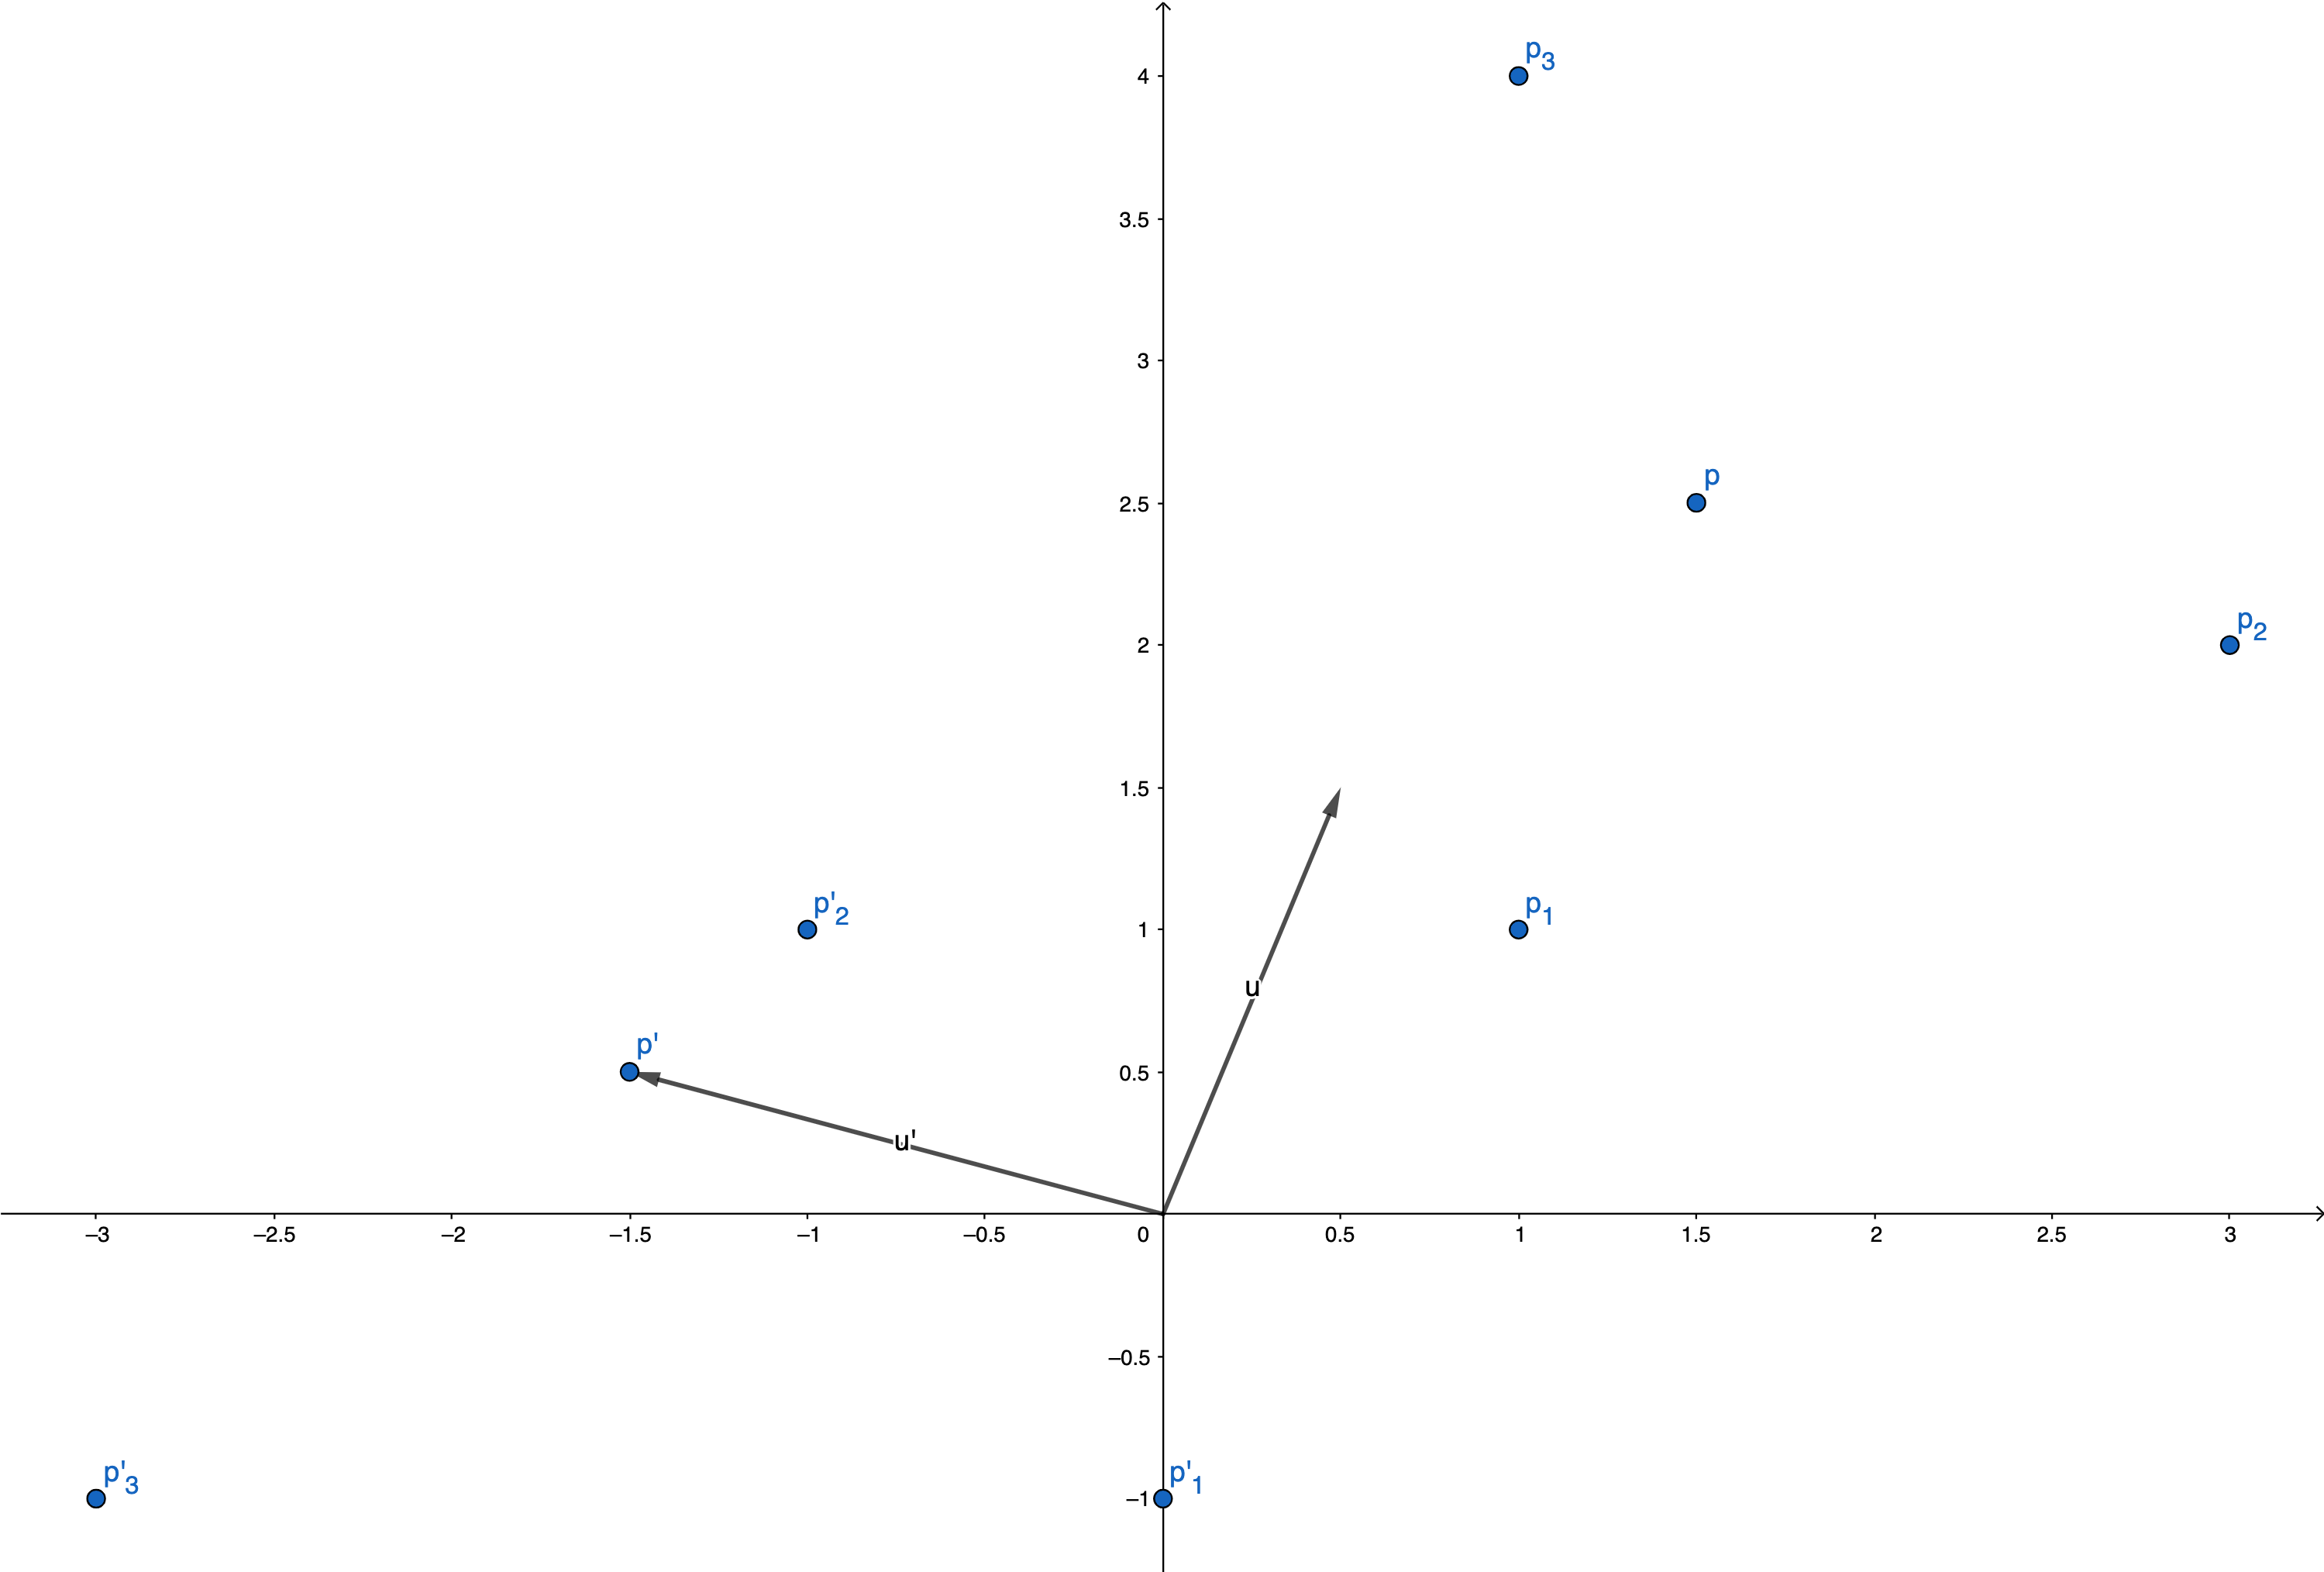
\includegraphics[width=14cm]{task_2.png}
\end{center}

\end{document}